\documentclass[a4paper,10pt]{article}

\usepackage[T1]{fontenc}
\usepackage[utf8]{inputenc}
\usepackage{graphicx}
\usepackage{xcolor}
\usepackage{float}

\usepackage{hyperref}

\hypersetup{
    %bookmarks=true,         % show bookmarks bar?
    unicode=false,          % non-Latin characters in Acrobat’s bookmarks
    pdftoolbar=true,        % show Acrobat’s toolbar?
    pdfmenubar=true,        % show Acrobat’s menu?
    pdffitwindow=false,     % window fit to page when opened
    pdfstartview={FitH},    % fits the width of the page to the window
    pdftitle={My title},    % title
    pdfauthor={Author},     % author
    pdfsubject={Subject},   % subject of the document
    pdfcreator={Creator},   % creator of the document
    pdfproducer={Producer}, % producer of the document
    pdfkeywords={keyword1, key2, key3}, % list of keywords
    pdfnewwindow=true,      % links in new PDF window
    colorlinks=true,       % false: boxed links; true: colored links
    linkcolor=red,          % color of internal links (change box color with linkbordercolor)
    citecolor=green,        % color of links to bibliography
    filecolor=magenta,      % color of file links
    urlcolor=blue           % color of external links
}

\renewcommand\familydefault{\sfdefault}
\usepackage{tgheros}
\usepackage[defaultmono]{droidmono}

\usepackage{amsmath,amssymb,amsthm,textcomp}
\usepackage{enumerate}
\usepackage{multicol}

\usepackage{tikz}
\usetikzlibrary{shadows,calc}
\def\shadowshift{3pt,-3pt}
\def\shadowradius{6pt}

\colorlet{innercolor}{black!60}
\colorlet{outercolor}{gray!05}

% this draws a shadow under a rectangle node
\newcommand\drawshadow[1]{
    \begin{pgfonlayer}{shadow}
        \shade[outercolor,inner color=innercolor,outer color=outercolor] ($(#1.south west)+(\shadowshift)+(\shadowradius/2,\shadowradius/2)$) circle (\shadowradius);
        \shade[outercolor,inner color=innercolor,outer color=outercolor] ($(#1.north west)+(\shadowshift)+(\shadowradius/2,-\shadowradius/2)$) circle (\shadowradius);
        \shade[outercolor,inner color=innercolor,outer color=outercolor] ($(#1.south east)+(\shadowshift)+(-\shadowradius/2,\shadowradius/2)$) circle (\shadowradius);
        \shade[outercolor,inner color=innercolor,outer color=outercolor] ($(#1.north east)+(\shadowshift)+(-\shadowradius/2,-\shadowradius/2)$) circle (\shadowradius);
        \shade[top color=innercolor,bottom color=outercolor] ($(#1.south west)+(\shadowshift)+(\shadowradius/2,-\shadowradius/2)$) rectangle ($(#1.south east)+(\shadowshift)+(-\shadowradius/2,\shadowradius/2)$);
        \shade[left color=innercolor,right color=outercolor] ($(#1.south east)+(\shadowshift)+(-\shadowradius/2,\shadowradius/2)$) rectangle ($(#1.north east)+(\shadowshift)+(\shadowradius/2,-\shadowradius/2)$);
        \shade[bottom color=innercolor,top color=outercolor] ($(#1.north west)+(\shadowshift)+(\shadowradius/2,-\shadowradius/2)$) rectangle ($(#1.north east)+(\shadowshift)+(-\shadowradius/2,\shadowradius/2)$);
        \shade[outercolor,right color=innercolor,left color=outercolor] ($(#1.south west)+(\shadowshift)+(-\shadowradius/2,\shadowradius/2)$) rectangle ($(#1.north west)+(\shadowshift)+(\shadowradius/2,-\shadowradius/2)$);
        \filldraw ($(#1.south west)+(\shadowshift)+(\shadowradius/2,\shadowradius/2)$) rectangle ($(#1.north east)+(\shadowshift)-(\shadowradius/2,\shadowradius/2)$);
    \end{pgfonlayer}
}

\pgfdeclarelayer{shadow} 
\pgfsetlayers{shadow,main}

\newcommand\shadowimage[2][]{%
\begin{tikzpicture}
\node[anchor=south west,inner sep=0] (image) at (0,0) {\includegraphics[#1]{#2}};
\drawshadow{image}
\end{tikzpicture}}

\usepackage{geometry}
\geometry{
    total={210mm,297mm},%
    left=25mm,right=25mm,%
    bindingoffset=0mm,%
    top=20mm,bottom=20mm%
}

\linespread{1.3}

\newcommand{\linia}{\rule{\linewidth}{0.5pt}}

\newtheoremstyle{mytheor}
    {1ex}{1ex}{\normalfont}{0pt}{\scshape}{.}{1ex}
    {{\thmname{#1 }}{\thmnumber{#2}}{\thmnote{ (#3)}}}

\theoremstyle{mytheor}
\newtheorem{defi}{Definici\'on}

\renewcommand{\tablename}{Tabla}
\renewcommand{\figurename}{Figura}

\makeatletter
\renewcommand{\maketitle}{
    \begin{center}
        \vspace{2ex}
        {\huge \textsc{\@title}}
        \vspace{1ex} \\
        \linia \\
        \hfill \@date  \\ 
        \@author
        \vspace{4ex}
    \end{center}
}
\makeatother
%%%

\usepackage{fancyhdr}
\pagestyle{fancy}
\lhead{}
\chead{}
\rhead{}
\lfoot{{\scriptsize Programaci\'on 2}}
\cfoot{}
\rfoot{P\'ag. \thepage}
\renewcommand{\headrulewidth}{0pt}
\renewcommand{\footrulewidth}{0pt}
%

% code listing settings
\usepackage{listings}
\lstset{
    language=Java,
    basicstyle=\ttfamily\small,
    aboveskip={1.0\baselineskip},
    belowskip={1.0\baselineskip},
    columns=fixed,
    extendedchars=true,
    breaklines=true,
    tabsize=4,
    prebreak=\raisebox{0ex}[0ex][0ex]{\ensuremath{\hookleftarrow}},
    frame=lines,
    showtabs=false,
    showspaces=false,
    showstringspaces=false,
    keywordstyle=\color[rgb]{0.627,0.126,0.941},
    commentstyle=\color[rgb]{0.133,0.545,0.133},
    stringstyle=\color[rgb]{01,0,0},
    numbers=left,
    numberstyle=\small,
    stepnumber=1,
    numbersep=10pt,
    captionpos=t,
    escapeinside={\%*}{*)}
}

%%%----------%%%----------%%%----------%%%----------%%%

\begin{document}

\title{{\huge Programaci\'on 2}}

\date{7 de junio de 2017}

\author{Profesor: \textbf{Rodrigo Olivares} (\href{mailto:rodrigo.olivares@uv.cl}{rodrigo.olivares@uv.cl}) \\ Escuela de Ingenier\'ia Civil  Inform\'atica \\ Universidad de Valpara\'iso \\}

\maketitle

\section{Descripci\'on de la tarea}

\begin{itemize}
    \item Individual \'o 2 personas (m\'aximo).
    \item Formato de informe IEEE: Resumen, Introducci\'on, Problema, Desarrollo y Conclusiones.
\end{itemize}

\subsection{Transformaci\'on de lenguajes}

Se debe realizar una aplicaci\'on en Java que permita transformar una o varias palabras, a diferentes lenguajes: alfabeto latino, alfabeto ascii y alfabeto morse. Para ello se pide los siguiente:

\begin{itemize}
    \item El usuario pueda ingresar un texto en cualquiera de los tres lenguajes.
    \item El usuario puede seleccionar un archivo de texto como dato de entrada.
    \item El sistema debe proporcionar la alternativa para seleccionar el lenguaje al que se desea transformar. 
    \item El sistema debe transformar la o las palabras y luego mostrarlas en alg\'un componente. De no ser posible realizar la transformaci\'on, el sistema debe informar al usuario que no se realiz\'o y porqu\'e.
    \item Al momento de transformar, el sistema deber\'a registrar la acci\'on, almacenando el resultado en un archivo de texto.
\end{itemize}

Una tentativa de interfaz gr\'afica de usuario puede ser vista en la Figura \ref{fig:v1}. El usuario puede ingresar un texto en el componente \texttt{JTextArea} o bien puede presionar el bot\'on \texttt{buscar} para abrir una ventana de di\'alogo, como se muestra en la Figura \ref{fig:v2}. Para desplegar este componente, se debe utilizar la clase \texttt{JFileChooser}\footnote{\url{http://docs.oracle.com/javase/7/docs/api/javax/swing/JFileChooser.html}}. Luego de ingresado el texto, el usuario debe seleccionar el lenguaje al cual se desea transformar, para finalmente, presionar el bot\'on \texttt{transformar}. Si el usuario presiona el bot\'on \texttt{transformar} sin seleccionar previamente el lenguaje, el sistema debe desplegar un mensaje de error, como se muestra en el Figura \ref{fig:v3}.

Al momento de transformar la o las palabras ingresadas, el sistema desplegar\'a el resultado en un componente. Luego, revisar\'a el estado del componente \texttt{JCheckBox}. Si est\'a activo, se almacenar\'a el resultado en un archivo de texto, con extensi\'on\texttt{.latin}, \texttt{.morse} o \texttt{.ascii}, si se transform\'o al alfabeto lat\'in, al alfabeto morse o al alfabeto ascii, respectivamente. El nombre del archivo debe ser din\'amico. Re recomienda utilizar la clase \texttt{Date} del package \texttt{java.util}.

Las Tablas \ref{tab:t1} y \ref{tab:t2}, muestran la equivalencia entre los lenguajes morse-lat\'in y ascii-lat\'in. Para ambos casos, la transformaci\'on s\'olo incluye los caracteres de la A a la Z, los d\'igitos del 0 al 9 y los s\'imboles punto, coma e interrogaci\'on (\texttt{.,?}). Para el caso de las letras, la transformaci\'on debe considerar s\'olo los elementos en may\'uscula, pues no existe equivalencia para m\'inuscula. %Se recomienda usar el m\'etodo \texttt{toUpperCase()} de la clase \texttt{String}, antes de realizar la transformaci\'on. 

\begin{figure}[H]
    \begin{center}
        \caption{Ejemplo ventana principal}\label{fig:v1}
        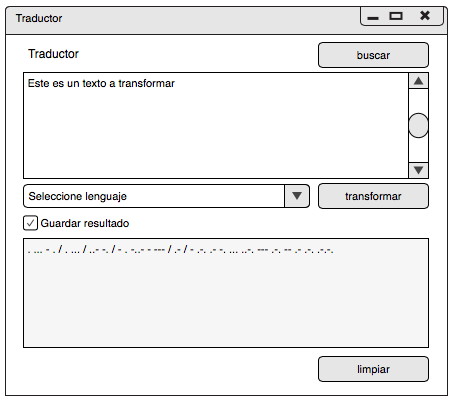
\includegraphics[scale=.65]{v1.png}
    \end{center}
\end{figure}

\begin{figure}[H]
    \begin{center}
        \caption{Ejemplo di\'alogo de selecci\'on de archivo}\label{fig:v2}
        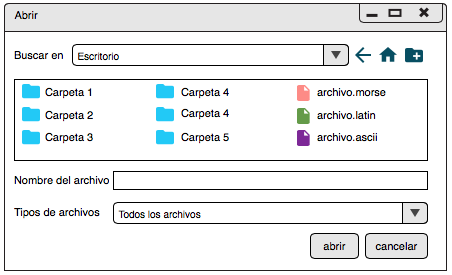
\includegraphics[scale=.65]{v2.png}
    \end{center}
\end{figure}

\begin{figure}[H]
    \begin{center}
        \caption{Ejemplo di\'alogo de error}\label{fig:v3}
        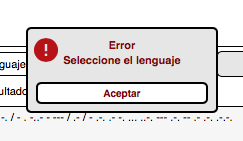
\includegraphics[scale=.65]{v3.png}
    \end{center}
\end{figure}

\begin{table}[H]
    \begin{center}
        \caption{Equivalencia morse-lat\'in}\label{tab:t1}
        \begin{tabular}{|c|c|c|c|c|c|} \hline
			\textbf{Signo} & \textbf{C\'odigo} & \textbf{Signo} & \textbf{C\'odigo} & \textbf{Signo} & \textbf{C\'odigo} \\ \hline
			A & $\cdot$-    & N & -$\cdot$ & 0 & - - - - -   \\ \hline
			B & -$\cdot\cdot\cdot$ & O & - - -   & 1 & $\cdot$- - - -   \\ \hline
			C & -$\cdot$-$\cdot$ & P & $\cdot$- -$\cdot$ & 2 & $\cdot\cdot$- - -   \\ \hline
			D & -$\cdot\cdot$   & Q & - -$\cdot$- & 3 & $\cdot\cdot\cdot$- -   \\ \hline
			E & $\cdot$ 	    & R & $\cdot$-$\cdot$   & 4 &	$\cdot\cdot\cdot\cdot$-   \\ \hline
			F & $\cdot\cdot$-$\cdot$ & S & $\cdot\cdot\cdot$   & 5 & $\cdot\cdot\cdot\cdot\cdot$   \\ \hline
			G & - -$\cdot$   & T & - 	  & 6 & -$\cdot\cdot\cdot\cdot$   \\ \hline
			H & $\cdot\cdot\cdot\cdot$ & U & $\cdot\cdot$-   & 7 & - -$\cdot\cdot\cdot$   \\ \hline
			I & $\cdot\cdot$     & V & $\cdot\cdot\cdot$- & 8 &	- - -$\cdot\cdot$   \\ \hline
			J & $\cdot$- - - & W & $\cdot$- -   & 9 &	- - - -$\cdot$   \\ \hline
			K & -$\cdot$-   & X & -$\cdot\cdot$- & . &	$\cdot$-$\cdot$-$\cdot$- \\ \hline
			L & $\cdot$-$\cdot\cdot$ & Y & -$\cdot$- - & , &	- -$\cdot\cdot$ - - \\ \hline
			M & - -     & Z & - -$\cdot\cdot$ & ? & $\cdot$- -$\cdot\cdot$   \\ \hline
		\end{tabular}
    \end{center}
\end{table}

\begin{table}[H]
    \begin{center}
        \caption{Equivalencia ascii-lat\'in}\label{tab:t2}
        \begin{tabular}{|c|c|c|c|c|c|} \hline
            \textbf{Signo} & \textbf{C\'odigo} & \textbf{Signo} & \textbf{C\'odigo} & \textbf{Signo} & \textbf{C\'odigo} \\ \hline
            0&\&\#48;	& D&\&\#68; & Q&\&\#81;	 \\ \hline
            1&\&\#49;	& E&\&\#69; & R&\&\#82;	 \\ \hline
            2&\&\#50;	& F&\&\#70; & S&\&\#83;	\\\hline
            3&\&\#51;	& G&\&\#71; & T&\&\#84;	 \\\hline
            4&\&\#52;	& H&\&\#72; & U&\&\#85;	 \\\hline
            5&\&\#53;	& I&\&\#73; & V&\&\#86;	 \\\hline
            6&\&\#54;	& J&\&\#74; & W&\&\#87;	\\\hline
            7&\&\#55;	& K&\&\#75; & X&\&\#88;	 \\\hline
            8&\&\#56;	& L&\&\#76; & Y&\&\#89;  \\\hline
            9&\&\#57;	& M&\&\#77; & Z&\&\#90;	 \\\hline
            A&\&\#65;	& N&\&\#78; & . &\&\#46;	 \\\hline
            B&\&\#66;	& O&\&\#79; & , &\&\#44;	 \\\hline
            C&\&\#67; & P&\&\#80; & ? &\&\#63;	 \\ \hline
		\end{tabular}
    \end{center}
\end{table}

\subsection{Entrega}

Deben entregar los archivos fuente \texttt{.java} y todo recurso utilizado por la aplicaci\'on, por ejemplo archivos, bibliotecas externas, etc. Se pondr\'a a disposici\'on un recurso \texttt{tarea} en el aula virtual, donde deber\'an subir un archivo \texttt{.zip} con el formato: 

\begin{center}
\texttt{ApellidoPaternoAlumno1ApellidoPaternoAlumno2.zip}
\end{center}
 
\noindent
En dicho archivo comprimido, deber\'an adjuntar el informe en formato PDF. La evaluaci\'on ser\'a: 65\% la aplicaci\'on y 35\% el informe. Deben utilizar todo lo visto en clases.\\

\noindent
\textbf{La fecha de entrega es el d\'ia martes 27 de junio, hasta las 12.00 hrs.}

\end{document}